\chapter{Аналитическая часть}

В данной части происходит анализ предметной области, обзор существующих аналогов,
формализация хранимой информации, формулировка требований и ограничений,
представлены ER-диаграмма сущностей, описание пользователей
и диаграмма вариантов использования.

\section{Анализ предметной области}

В современном мире наборы данных (датасеты) стали основой для анализа,
машинного обучения, научных исследований и бизнес-аналитики. Под датасетом понимается структурированная коллекция данных,
используемая для анализа, обработки или обучения моделей машинного обучения.
Датасет состоит из наблюдений (экземпляров) и признаков (характеристик), которые описывают каждое наблюдение.
Такие наборы данных используются как входная информация для алгоритмов и моделей, а также для повторного анализа,
тестирования и воспроизведения научных результатов~\cite{intro1}.

На практике хранение и управление датасетами осуществляется с использованием как специализированных
онлайн-платформ (например, Kaggle~\cite{kaggle}, Hugging Face~\cite{hg}, ClearML~\cite{cml}), так и в
локальных файловых системах.
При этом часто возникают проблемы, связанные с отсутствием единых стандартов хранения, невозможностью эффективно
отслеживать версии, а также слабо реализованной системой доступа по ролям.
Это приводит к потере актуальности данных, дублированию и затруднениям в повторном использовании~\cite{bp}.

Для систем хранения датасетов важно учитывать следующие аспекты:
\begin{itemize}
    \item версионирование — возможность сохранять историю изменений и откатываться к предыдущим версиям;

    \item метаданные — структурированная информация о датасете (описание, автор, дата создания, ключевые слова и пр.);

    \item связь с файлами — каждый датасет может состоять из одного или нескольких файлов разных форматов;

    \item права доступа — разграничение доступа для разных категорий пользователей (например, гостевой просмотр, авторское редактирование, администрирование);

    \item категоризация — удобная система разделения по категориям.
\end{itemize}

\section{Анализ существующих решений}

Для выявления ключевых требований к системе хранения и управления наборами данных, был проведён анализ 
четырёх популярных платформ: Kaggle, Hugging Face Datasets, UCI Machine Learning Repository и ClearML. 
Каждая из этих платформ имеет свою специфику, ориентирована на разные аудитории и задачи, и реализует 
различные подходы к организации данных.

%\begin{enumerate}
%    \item Kaggle datasets --- платформа для проведения соревнований по анализу данных, а также для обмена датасетами и ноутбуками~\cite{kaggle};
%    \item Hugging Face Datasets --- открытая платформа для обмена и использования датасетов~\cite{hg};
%    \item UCI Machine Learning Repository --- один из старейших репозиториев, основной упор сделан на академические датасеты~\cite{uci};
%    \item ClearML — платформа для управления ML-проектами, которая поддерживает загрузку, версионирование и отслеживание датасетов в рамках ML-пайплайнов~\cite{cml}.
%\end{enumerate}

\begin{enumerate}
    \item \textbf{Kaggle Datasets} --- платформа для проведения соревнований по анализу данных, а также для обмена наборами данных~\cite{kaggle};

    \item \textbf{Hugging Face Datasets} --- открытая платформа для хранения, загрузки и использования наборов данных, преимущественно в области обработки естественного языка~\cite{hg};

    \item \textbf{UCI Machine Learning Repository} --- один из старейших репозиториев академических наборов дынных, ориентирован на предоставление исходных файлов для загрузки~\cite{uci};

    \item \textbf{ClearML} — платформа для управления процессами машинного обучения с возможностью отслеживания экспериментов и хранения наборов данных~\cite{cml}.
\end{enumerate}

Критерии, выделенные для сравнения существующих решений:

\begin{itemize}
    \item \textbf{Поддержка версий} — возможность хранения нескольких версий одного и того же датасета с отслеживанием изменений и восстановлением предыдущих состояний;

    \item \textbf{Отзывы и оценки} — наличие системы рейтингов, комментариев и обратной связи от пользователей, позволяющей оценивать качество и актуальность данных;

    \item \textbf{Уведомления об обновлениях} — рассылка автоматических оповещений о появлении новых версий датасетов подписанным пользователям;

    \item \textbf{Доступ к публичным датасетам} — наличие открытого доступа к общедоступным наборам данных без необходимости регистрации или подтверждения прав доступа.
\end{itemize}

\begin{table}[H]
\centering
\caption{Сравнение существующих платформ хранения датасетов}
\begin{tabular}{|l|c|c|c|c|}
\hline
\textbf{Платформа} &
\makecell{\textbf{Версио-} \\ \textbf{нирование}} &
\makecell{\textbf{Публичные} \\ \textbf{датасеты}} &
\makecell{\textbf{Отзывы и} \\ \textbf{оценки}} &
\makecell{\textbf{Уведомления об} \\ \textbf{обновлении}} \\
\hline
Kaggle & Нет & Да & Да & Нет \\
\hline
Hugging Face & Да & Да & Нет & Нет \\
\hline
UCI & Нет & Да & Нет & Нет \\
\hline
ClearML & Да & Нет & Нет & Да \\
\hline
\end{tabular}
\end{table}

Ни одно из вышеперечисленных существующих решений не удовлетворяет всем упомянутым критериям.
Таким образом, отличием разрабатываемой системы является обеспечение всех выделенных критериев,
что делает её универсальной и удобной для пользователей.

\section{Анализ моделей данных}

В данном разделе проводится обзор основных моделей данных,
что необходимо для аргументированного выбора оптимального решения при разработке системы хранения и
управления датасетами.

База данных – это самодокументированное собрание интегрированных записей.
Под самодокументированностью базы данных понимается наличие в её составе метаданных — информации,
описывающей структуру и организацию самих данных, включая таблицы, поля,
типы данных и связи между сущностями.
Интегрированность записей означает, что данные в базе логически связаны, согласованы и хранятся совместно с элементами,
обеспечивающими их целостность и оптимальный доступ, такими как индексы и служебные структуры,
описывающие взаимодействие с прикладными компонентами.~\cite{BD}

Система управления базами данных (СУБД) --- это набор программ, которые управляют
структурой БД и контролируют доступ к данным, хранящимся в БД.

Логическая модель базы данных --- версия структуры данных, на основе которой реализована конкретная СУБД.

По модели данных СУБД делятся на дореляционные, реляцирнные и постреляционные.~\cite{data_model}

\subsubsection*{Дореляционные модели}

Дореляционные модели баз данных, к которым относятся иерархическая и сетевая, стали предшественниками реляционного подхода.
В этих системах доступ к информации осуществлялся на уровне отдельных записей,
и пользователи были вынуждены явно задавать маршруты навигации по структурам данных, как правило,
через расширения языков программирования.~\cite{dorel}

Иерархическая модель представляла данные в виде древовидных структур с жёсткими связями «предок–потомок»,
что хорошо подходило для описания естественно иерархичных объектов.
Сетевая модель, в свою очередь, расширила этот подход, позволив потомкам иметь несколько предков и тем
самым лучше отражать сложные взаимосвязи между данными.
Несмотря на появление реляционных систем, отдельные реализации дореляционных моделей сохраняют актуальность
благодаря своей эффективности в специфических областях.~\cite{dorel}

Преимуществом дореляционных моделей является близость к естественным способам организации данных,
что обеспечивало их эффективность в прикладных областях.
Недостатком же являлась необходимость навигации на уровне отдельных записей и отсутствие развитых средств
декларативного доступа.

\subsubsection*{Реляционные модели}

Реляционные базы данных получили широкое распространение благодаря удобству представления информации в виде таблиц,
состоящих из строк и столбцов, и применению строгого математического аппарата реляционной алгебры.
Основные свойства реляционной модели включают уникальность строк, однородность данных в столбцах,
наличие уникальных имён атрибутов и независимость порядка строк и столбцов.
Такой подход обеспечивает простоту использования и гибкость в организации связей типа «один к одному» и «один ко многим».

Преимуществом реляционной модели является её универсальность и удобство декларативного доступа к данным,
что позволило создать на её основе большинство современных СУБД.
К ограничениям можно отнести снижение эффективности при работе с очень большими объёмами данных и необходимость
сложной оптимизации запросов, что стимулировало развитие постреляционных решений.~\cite{rel}

\subsubsection*{Постреляционные модели}

Постреляционная модель представляет собой дальнейшее развитие реляционного подхода и снимает ограничение на неделимость
данных.
В отличие от классической реляционной модели, она допускает использование многозначных полей,
каждое из которых может содержать множество значений и рассматриваться как вложенная таблица.
Это обеспечивает повышенную гибкость структуры данных, поскольку длина и количество полей в записях не фиксированы.

Основным преимуществом постреляционной модели является возможность объединения нескольких связанных реляционных таблиц
в единую структуру, что делает представление информации более наглядным и повышает эффективность её обработки.
Вместе с тем к недостаткам относятся сложности в обеспечении целостности и согласованности данных,
что усложняет практическую реализацию таких систем.~\cite{dorel}

\subsubsection*{Выбор модели данных}

Для реализации системы хранения датасетов целесообразно использовать комбинированный подход.
Сами датасеты представляют собой крупные файлы различных форматов и хранятся во внешнем объектном хранилище,
оптимизированном для работы с неструктурированными данными.
Однако информация о них --- сведения о версиях, категориях, тегах и пользователях, требуют строгой структуризации и
поэтому размещаются в реляционной базе данных, обеспечивающей целостность и удобный декларативный доступ.


\section{Формализация задачи}

Необходимо спроектировать базу данных для хранения информации о датасетах, их версиях, связанных файлах,
метаданных, тегах, категориях и пользователях. Требуется разработать приложение, предоставляющее интерфейс для просмотра,
загрузки, редактирования и удаления информации, хранящейся в базе данных.
Необходимо реализовать три вида ролей — гость, авторизованный пользователь и администратор.

В рамках поставленной цели необходимо спроектировать и реализовать базу данных,
содержащую информацию о датасетах и их структуре, поддерживающую версионирование, управление доступом и систему
уведомлений об обновлениях. Приложение должно обеспечить возможность ведения метаданных и
отслеживания изменений, а также предоставлять пользователю удобный интерфейс для взаимодействия с данными в рамках его
роли.

\section{Формализация данных}

На основании ER-диаграммы были выделены следующие основные категории данных:

\begin{itemize}
  \item Пользователи
  \item Подписки
  \item Категории
  \item Датасеты
  \item Версии датасетов
  \item Метаданные
  \item Отзывы
\end{itemize}

\begin{table}[H]
\centering
\caption{Формализация сущностей и их атрибутов}
\renewcommand{\arraystretch}{1.4}
\begin{tabular}{|l|p{10cm}|}
\hline
\textbf{Категория} & \textbf{Сведения о данных (атрибуты)} \\
\hline
Пользователь &
Идентификатор, Имя пользователя, Пароль, Электронная почта, Страна, Дата регистрации \\
\hline
Категория &
Идентификатор, Название, Описание \\
\hline
Датасет &
Идентификатор, Название, Описание, Уровень доступа, Дата создания, Владелец, Категория \\
\hline
Подписка &
Идентификатор, Дата создания, Датасет, Пользователь \\
\hline
Версия датасета &
Идентификатор, Идентификатор датасета, Номер версии, Дата загрузки, Путь к файлу \\
\hline
Метаданные &
Идентификатор, Идентификатор датасета, Формат, Размер, Теги \\
\hline
Отзыв &
Идентификатор, Пользователь, Датасет, Текст отзыва, Оценка \\
\hline
\end{tabular}
\end{table}


На рисунке~\ref{img:er} приведена ER-диаграмма сущностей в нотации Чена.

\begin{figure}[H]
	\centering
	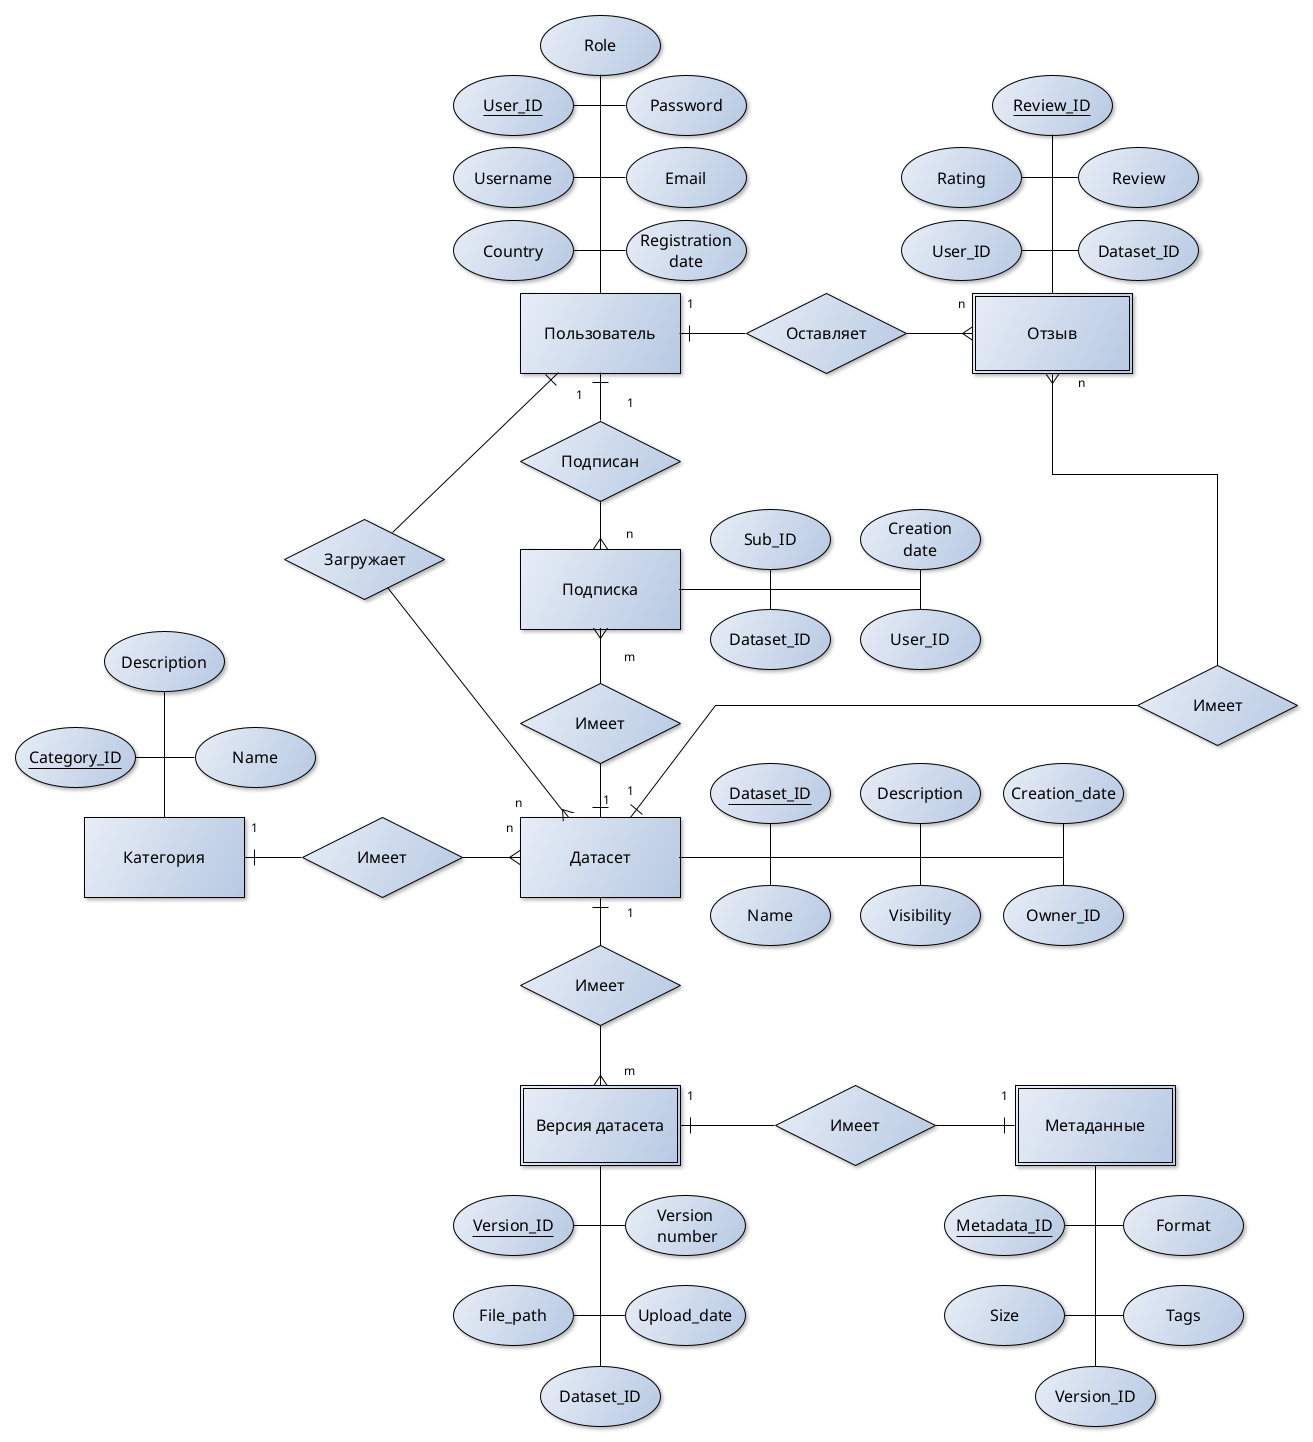
\includegraphics[scale=0.3]{images/er}
	\caption{ER-диаграмма сущностей в нотации Чена}
	\label{img:er}
\end{figure}

\section{Формализация ролей}

Следует выделить группы пользователей разрабатываемой системы, исходя из
предметной области поставленной задачи:

\begin{itemize}
    \item гость --- неавторизованный пользователь, который имеет возможность просматривать публичные датасеты и их метаданные а также скачивать их;
    \item авторизованный пользователь --- пользователь, прошедший процедуру регистрации и авторизации. Может загружать собственные датасеты, редактировать их метаданные, создавать новые версии;
    \item администратор --- обладает полными правами для управления всеми датасетами, метаданными, а также управляет правами доступа других пользователей, модерирует контент и контролирует работу системы.
\end{itemize}

На рисунке~\ref{img:ucase} приведена диаграмма вариантов использования.

\begin{figure}[H]
	\centering
	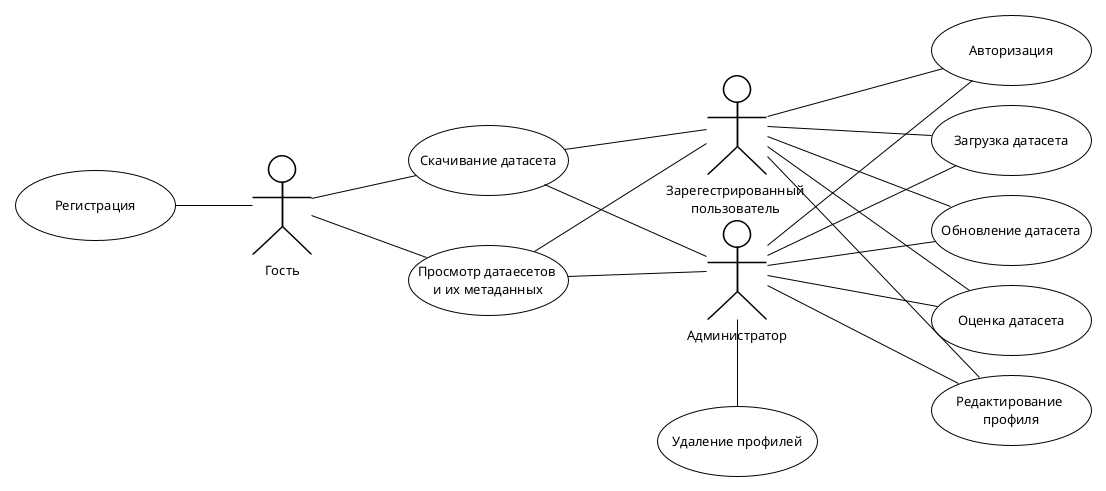
\includegraphics[scale=0.35]{images/use_case}
	\caption{Use-case диаграмма.}
	\label{img:ucase}
\end{figure}


\section*{Вывод}

В данном разделе была проанализирована предметная область, поставленная задача и рассмотрены существующие решения
по хранению и управлению датасетами. Проведено сравнение популярных платформ, выявлены их достоинства и недостатки,
а также сформулированы ключевые требования к разрабатываемой системе. Поскольку задача предполагает хранение
взаимосвязанных структурированных данных, поддержку версионирования, отзывов, тегов и различных ролей пользователей,
приоритетными свойствами модели данных являются целостность, расширяемость и независимость от пользовательского интерфейса.